\documentclass[14pt]{extarticle}
\usepackage{fontspec}
\usepackage{polyglossia}
\usepackage{amsmath}
\usepackage{amssymb}
\usepackage{xcolor}
\usepackage{fancyhdr}
\usepackage{graphicx}
\usepackage{listings}
\usepackage[most]{tcolorbox}
% \usepackage{setspace}
\usepackage{pifont}
\usepackage{enumitem}
\usepackage{titlesec}
\usepackage[bottom]{footmisc}
\usepackage{titling}
\usepackage{minted}
\usepackage{etoolbox}
\usepackage{array}
\usepackage{extsizes}
\usepackage{float}
\usepackage{booktabs}
\usepackage{hyperref}
\usepackage[onehalfspacing]{setspace}
\usepackage[a4paper, top=2.7cm, bottom=2.7cm, left=2.5cm, right=2.5cm, headheight=1.5cm, headsep=0.5cm]{geometry}
\usepackage{tikz}

\usetikzlibrary{automata, positioning, arrows.meta, arrows}

\newfontfamily\emoji{Segoe UI Emoji}

\pagestyle{fancy}

\setmainlanguage[numerals=western]{arabic}
\setotherlanguage{english}
% \newfontfamily\arabicfont[Script=Arabic]{Amiri}
\newfontfamily\arabicfont[Script=Arabic]{Calibri}
\newfontfamily\arabicfonttt[Script=Arabic]{Courier New}

\lstset{
  language=[Sharp]C,
  numbers=left,
  stepnumber=1,
  numbersep=8pt,
  frame=single,
  basicstyle=\ttfamily\small,
  keywordstyle=\color{blue},
  stringstyle=\color{red},
  commentstyle=\color{green!50!black}
}

\newif\ifdetailed
\ifdefined\setdetailed
  \setdetailed
\fi

\newif\ifwithsols
\ifdefined\setwithsols
  \setwithsols
\fi

% unified tcolorboxes for articles
\tcbset{colback=white, colframe=black, fonttitle=\bfseries, boxrule=0.8pt}
\newtcolorbox{boxDef}[1][]{colback=blue!5!white,colframe=blue!75!black,
  title={{\emoji📘} تعريف\ifx\\#1\\\else ~#1\fi :}}
\newtcolorbox{boxExercise}[1][]{colback=cyan!5!white,colframe=cyan!70!black,
  title={{\emoji🧩} تمرين\ifx\\#1\\\else ~#1\fi :}}
\newtcolorbox{boxExample}[1][]{colback=yellow!5!white,colframe=orange!90!black,
  title={{\emoji📝} مثال\ifx\\#1\\\else ~#1\fi :}}
\newtcolorbox{boxNote}[1][]{colback=gray!10!white,colframe=black,
  title={{\emoji✨} ملاحظة\ifx\\#1\\\else ~#1\fi :}}
\newtcolorbox{boxAttention}[1][]{colback=magenta!10!white,colframe=magenta!80!black,
  title={{\emoji🔔} تنبيه\ifx\\#1\\\else ~#1\fi :}}
\newtcolorbox{boxWarning}[1][]{colback=red!5!white,colframe=red!75!black,
  title={{\emoji⚡} ملاحظة هامة\ifx\\#1\\\else ~#1\fi :}}
\newtcolorbox{boxSolution}[1][]{colback=green!5!white,colframe=green!60!black,
  title={{\emoji✅} حل\ifx\\#1\\\else ~#1\fi :}}
\newtcolorbox{boxSymbol}[1][]{colback=purple!5!white,colframe=purple!70!black,
  title={{\emoji🔣} رمز\ifx\\#1\\\else ~#1\fi :}}
\newtcolorbox{boxHint}[1][]{colback=teal!5!white,colframe=teal!60!black,
  title={{\emoji💡} تلميح\ifx\\#1\\\else ~#1\fi :}}


\tcbset{simplecode/.style={ colback=gray!5, colframe=black!50, boxrule=0.4pt, arc=2pt, left=4pt,right=4pt,top=4pt,bottom=4pt}}
\newenvironment{boxCode}{\begin{tcolorbox}[simplecode]}{\end{tcolorbox}}

\newcolumntype{C}[1]{>{\centering\arraybackslash}p{#1}}

% redefine spaces after titles
\makeatletter
\renewcommand{\@maketitle}{%
  \begin{center}
    {\huge \bfseries \@title \par}%
    \vskip 0.2em % space between title and author
    {\large \@author \par}%
    % \vskip 0.2em % space between author and date
    % {\normalsize \@date \par}%
  \end{center}
}
\makeatother

\fancyhf{} % clear default
\fancypagestyle{plain}{
  \fancyhf{}
  \fancyhead[L]{مدرسة التسامح الشاملة}
  % \fancyhead[L]{
\includegraphics[height=1cm]{../../../images/logoTasamoh.png}}
  \fancyhead[R]{الأستاذ محمود اغبارية}
  \fancyfoot[C]{\thepage}
}

\fancyhead[L]{مدرسة التسامح الشاملة}
\fancyhead[R]{الأستاذ محمود اغبارية}
\fancyfoot[C]{\thepage}
% \date{\today}

\setcounter{tocdepth}{3} % only section subsection and subsubsection in TOC

\newcommand{\importpdfpage}[2]{%
    \thispagestyle{empty}
    \newgeometry{left=0cm,right=0cm,top=0cm,bottom=0cm}
    \includegraphics[page=#2,width=0.95\paperwidth,height=0.95\paperheight,keepaspectratio]{#1}
    \restoregeometry
}

\newcommand{\insertFullImg}[1]{%
    \noindent
    \makebox[\textwidth][c]{
        \includegraphics[width=0.9\paperwidth,keepaspectratio]{#1}%
    }%
}%

% ----------------------


% \begin{document}

% \maketitle

% % \clearpage  % start TOC on a new page
% % \renewcommand{\contentsname}{جدول المحتويات}
% % \tableofcontents
% % \clearpage

% \part*{part 1} % the * prevents numbering
% \section*{مقدمة}
% \subsection*{مثال رياضي}
% \subsubsection*{مثال فرعي}
% \paragraph*{ paragraph 1}
% \subparagraph*{sub paragraph 1}

% \ifdetailed
% \begin{english}
% \begin{minted}{csharp}
% // C# Example
% \end{minted}
% \end{english}
% \fi

% OLD WAY
% \ifdetailed
% \begin{english}
% \begin{lstlisting}
% // C# Example
% \end{lstlisting}
% \end{english}
% \fi

% % 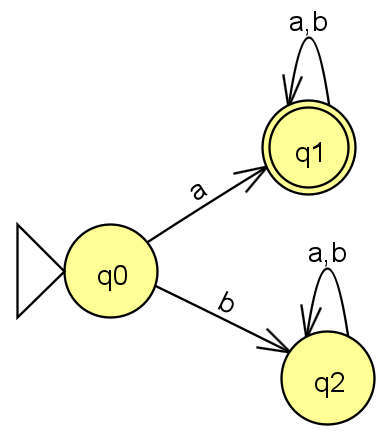
\includegraphics[width=0.2\textwidth]{../../../images/DFAs/ex1_q1.png}



% \vspace{3cm}
% \begin{flushleft}
% أرجو لكم وقتًا ممتعًا.

% الأستاذ محمود اغبارية.
% \end{flushleft}


% \end{document}


\ifwithsols
\title{حل ورقة تمرن 1 للصف العاشر 10}
\else
\title{ورقة تمرن 1 للصف العاشر 10}
\fi

\begin{document}

\maketitle
\thispagestyle{fancy}

\begin{enumerate}[itemsep=2em]

    % ------------------------------------------------------
    % 1. [New] Read and print
    % ------------------------------------------------------
    \item
    اكتب برنامجًا يستقبل من المستخدم رقمًا صحيحًا، ويطبع له نفس الرقم الذي أدخله. \\
    \textbf{مثال:} إذا أدخل المستخدم $5$، يطبع البرنامج $5$.
    \ifwithsols
    \begin{boxSolution}
    \begin{english}
    \begin{minted}{csharp}
int num = int.Parse(Console.ReadLine());
Console.WriteLine(num);
    \end{minted}
    \end{english}
    \end{boxSolution}
    \fi

    % ------------------------------------------------------
    % 2. [New] Multiply by 2
    % ------------------------------------------------------
    \item
    اكتب برنامجًا يستقبل من المستخدم رقمًا، ويطبع له ضعف هذا الرقم (أي الرقم مضروبًا بـ 2). \\
    \textbf{مثال:} إذا أدخل المستخدم $4$، يطبع البرنامج $8$.
    \ifwithsols
    \begin{boxSolution}
    \begin{english}
    \begin{minted}{csharp}
int num = int.Parse(Console.ReadLine());
Console.WriteLine(num * 2);
    \end{minted}
    \end{english}
    \end{boxSolution}
    \fi

    % ------------------------------------------------------
    % 3. [New] Previous and Next
    % ------------------------------------------------------
    \item
    اكتب برنامجًا يستقبل من المستخدم رقمًا صحيحًا، ويطبع له العدد الذي يسبقه والعدد الذي يليه. \\
    \textbf{مثال:} إذا أدخل المستخدم $10$، يطبع البرنامج $9$ ثم $11$.
    \ifwithsols
    \begin{boxSolution}
    \begin{english}
    \begin{minted}{csharp}
int num = int.Parse(Console.ReadLine());
Console.WriteLine(num - 1);
Console.WriteLine(num + 1);
    \end{minted}
    \end{english}
    \end{boxSolution}
    \clearpage
    \fi

    % ------------------------------------------------------
    % 4. [New] Square
    % ------------------------------------------------------
    \item
    اكتب برنامجًا يستقبل من المستخدم رقمًا، ويطبع له مربّع هذا الرقم (أي الرقم مضروبًا بنفسه). \\
    \textbf{مثال:} إذا أدخل المستخدم $5$، يطبع البرنامج $25$.
    \ifwithsols
    \begin{boxSolution}
    \begin{english}
    \begin{minted}{csharp}
int num = int.Parse(Console.ReadLine());
Console.WriteLine(num * num);
    \end{minted}
    \end{english}
    \end{boxSolution}
    \fi

    % ------------------------------------------------------
    % 5. [Old] Triangle Perimeter
    % ------------------------------------------------------
    \item
    اكتب برنامجًا يستقبل من المستخدم أطوال أضلاع مثلث ويطبع له محيط المثلث. \\
    (محيط المثلث = مجموع أطوال الأضلاع)
    \ifwithsols
    \begin{boxSolution}
    \begin{english}
    \begin{minted}{csharp}
int a = int.Parse(Console.ReadLine());
int b = int.Parse(Console.ReadLine());
int c = int.Parse(Console.ReadLine());
Console.WriteLine(a + b + c);
    \end{minted}
    \end{english}
    \end{boxSolution}
    \fi

\item
اكتب برنامجًا يستقبل من المستخدم طول ضلع مربّع ويطبع له مساحة المربّع ومحيطه.
$$ \text{Area} = side ^ 2 $$
$$ \text{Perimeter} = 4 \cdot side $$
\ifwithsols
\begin{boxSolution}
\begin{english}
\begin{minted}{csharp}
int side = int.Parse(Console.ReadLine());
int area = side * side;
int perimeter = 4 * side;
Console.WriteLine(area);
Console.WriteLine(perimeter);
\end{minted}
\end{english}
\end{boxSolution}
\clearpage
\fi

\item
اكتب برنامجا يستقبل من المستخدم طول قاعدة المثلث والارتفاع ويطبع له مساحة المثلث.
$$ \text{Area} = \frac{width \cdot height}{2} $$
\ifwithsols
\begin{boxSolution}
\begin{english}
\begin{minted}{csharp}
int width = int.Parse(Console.ReadLine());
int height = int.Parse(Console.ReadLine());
double area = width * height / 2.0;
Console.WriteLine(area);
\end{minted}
\end{english}
\end{boxSolution}
\fi

\item
اكتب برنامجًا يستقبل من المستخدم طول مستطيل وعرضه ويطبع له مساحة المستطيل ومحيطه.
$$ \text{Area} = width \cdot height $$
$$ \text{Perimeter} = 2 \cdot width + 2 \cdot height $$
\ifwithsols
\begin{boxSolution}
\begin{english}
\begin{minted}{csharp}
int width = int.Parse(Console.ReadLine());
int height = int.Parse(Console.ReadLine());
int area = width * height;
int perimeter = 2 * width + 2 * height;
Console.WriteLine(area);
Console.WriteLine(perimeter);
\end{minted}
\end{english}
\end{boxSolution}
\clearpage
\fi

\item
اكتب برنامجًا يستقبل من المستخدم طول نصف قطر دائرة، ويطبع له محيطها ومساحتها.
$$ \text{Area} = 3.14 \cdot r^2 $$
$$ \text{Perimeter} = 2 \cdot 3.14 \cdot r $$
\ifwithsols
\begin{boxSolution}
\begin{english}
\begin{minted}{csharp}
int r = int.Parse(Console.ReadLine());
double area = 3.14 * r * r;
double perimeter = 2 * 3.14 * r;
Console.WriteLine(area);
Console.WriteLine(perimeter);
\end{minted}
\end{english}
\end{boxSolution}
\fi

\item
اكتب برنامجًا يستقبل من المستخدم علامات 3 مواضيع: اللغة العربية، الرياضيات والحاسوب، ويطبع له معدّل العلامات الثلاث.
\ifwithsols
\begin{boxSolution}
\begin{english}
\begin{minted}{csharp}
int arabic = int.Parse(Console.ReadLine());
int math = int.Parse(Console.ReadLine());
int cs = int.Parse(Console.ReadLine());
double average = (arabic + math + cs) / 3.0;
Console.WriteLine(average);
\end{minted}
\end{english}
\end{boxSolution}
\clearpage
\fi

\item
اكتب برنامجًا يستقبل من المستخدم علامات 3 مواضيع: اللغة العربية، الرياضيات والحاسوب، ثم يستقبل منه عدد الوحدات لكل موضوع، ويطبع له معدّل العلامات الثلاث.
\ifwithsols
\begin{boxSolution}
\begin{english}
\begin{minted}{csharp}
int arabic = int.Parse(Console.ReadLine());
int math = int.Parse(Console.ReadLine());
int cs = int.Parse(Console.ReadLine());

int unitsArabic = int.Parse(Console.ReadLine());
int unitsMath = int.Parse(Console.ReadLine());
int unitsCs = int.Parse(Console.ReadLine());

int totalGrades = arabic * unitsArabic + math * unitsMath + cs * unitsCs;
int totalUnits = unitsArabic + unitsMath + unitsCs;
double average = (double)totalGrades / totalUnits;
Console.WriteLine(average);
\end{minted}
\end{english}
\end{boxSolution}
\fi

\item
اكتب برنامجًا يستقبل من المستخدم طوله بالمتر، ووزنه بالكغم، ويحسب له درجة الـ BMI حسب المعادلة التالية:
$$ \text{BMI} = \frac{weight}{height^2} $$
\ifwithsols
\begin{boxSolution}
\begin{english}
\begin{minted}{csharp}
double height = double.Parse(Console.ReadLine());
int weight = int.Parse(Console.ReadLine());
double bmi = weight / (height * height);
Console.WriteLine(bmi);
\end{minted}
\end{english}
\end{boxSolution}
\fi
\clearpage

\item
اكتب برنامجًا يستقبل من المستخدم درجة الحرارة بالدرجة المئوية، ويطبع له الدرجة بالفهرنهايت وبالكلفن حسب المعادلات التالية:
$$ F = \frac{9}{5} \times C + 32 $$
$$ K = C + 273.15 $$
\ifwithsols
\begin{boxSolution}
\begin{english}
\begin{minted}{csharp}
int c = int.Parse(Console.ReadLine());
double f = (9.0 / 5.0) * c + 32;
double k = c + 273.15;
Console.WriteLine(f);
Console.WriteLine(k);
\end{minted}
\end{english}
\end{boxSolution}
\fi

\item
اكتب برنامجًا يستقبل من المستخدم درجة الحرارة بالفهرنهايت، ويطبع له الدرجة بالدرجة المئوية حسب المعادلة التالية:
$$ C = \frac{5}{9} \times (F - 32) $$
\ifwithsols
\begin{boxSolution}
\begin{english}
\begin{minted}{csharp}
int f = int.Parse(Console.ReadLine());
double c = (5.0 / 9.0) * (f - 32);
Console.WriteLine(c);
\end{minted}
\end{english}
\end{boxSolution}
\fi

\item
اكتب برنامجًا يستقبل من المستخدم درجة الحرارة بالكلفن، ويطبع له الدرجة بالدرجة المئوية حسب المعادلة التالية:
$$ C = K - 273.15 $$
\ifwithsols
\begin{boxSolution}
\begin{english}
\begin{minted}{csharp}
int k = int.Parse(Console.ReadLine());
double c = k - 273.15;
Console.WriteLine(c);
\end{minted}
\end{english}
\end{boxSolution}
\fi

\item
اكتب برنامجًا يستقبل من المستخدم درجة الحرارة بالفهرنهايت، ويطبع له الدرجة بالكلفن حسب المعادلة التالية:
$$ K = \frac{5}{9} \times (F - 32) + 273.15 $$
\ifwithsols
\begin{boxSolution}
\begin{english}
\begin{minted}{csharp}
int f = int.Parse(Console.ReadLine());
double k = (5.0 / 9.0) * (f - 32) + 273.15;
Console.WriteLine(k);
\end{minted}
\end{english}
\end{boxSolution}
\fi

\item
اكتب برنامجًا يستقبل من المستخدم درجة الحرارة بالكلفن، ويطبع له الدرجة بالفهرنهايت حسب المعادلة التالية:
$$ F = \frac{9}{5} \times (K - 273.15) + 32 $$
\ifwithsols
\begin{boxSolution}
\begin{english}
\begin{minted}{csharp}
int k = int.Parse(Console.ReadLine());
double f = (9.0 / 5.0) * (k - 273.15) + 32;
Console.WriteLine(f);
\end{minted}
\end{english}
\end{boxSolution}
\clearpage
\fi

\item
اكتب برنامجًا يستقبل من المستخدم 5 أرقام، واحدًا تلوَ الآخر. في كل مرة يدخل المستخدم رقمًا جديدًا، يطبع له البرنامج مجموع الأرقام التي أدخلها المستخدم حتى الآن.
\ifwithsols
\begin{boxSolution}
\begin{english}
\begin{minted}{csharp}
int n1 = int.Parse(Console.ReadLine());
Console.WriteLine(n1);

int n2 = int.Parse(Console.ReadLine());
Console.WriteLine(n1 + n2);

int n3 = int.Parse(Console.ReadLine());
Console.WriteLine(n1 + n2 + n3);

int n4 = int.Parse(Console.ReadLine());
Console.WriteLine(n1 + n2 + n3 + n4);

int n5 = int.Parse(Console.ReadLine());
Console.WriteLine(n1 + n2 + n3 + n4 + n5);
\end{minted}
\end{english}
\end{boxSolution}
\clearpage
\fi

\item
حل السؤال السابق باستخدام متغيّرين فقط.
\ifwithsols
\begin{boxSolution}
\begin{english}
\begin{minted}{csharp}
int sum = 0;
int num;

num = int.Parse(Console.ReadLine());
sum = sum + num;
Console.WriteLine(sum);

num = int.Parse(Console.ReadLine());
sum = sum + num;
Console.WriteLine(sum);

num = int.Parse(Console.ReadLine());
sum = sum + num;
Console.WriteLine(sum);

num = int.Parse(Console.ReadLine());
sum = sum + num;
Console.WriteLine(sum);

num = int.Parse(Console.ReadLine());
sum = sum + num;
Console.WriteLine(sum);
\end{minted}
\end{english}
\end{boxSolution}
\fi

\end{enumerate}

\vspace{3cm}
\begin{flushleft}
أرجو لكم وقتًا ممتعًا.

الأستاذ محمود اغبارية.
\end{flushleft}

\end{document}
